\chapter{Concept \& Design}
In this chapter we describe the research problem and our solution. Regarding the solution we discuss 
the ML aspects of this research and the architectural design to get the ML models running in a real-time
environment.

\section{Problem Statement}
The rise of online tracking techniques poses significant privacy concerns for users while browsing the web.
Traditional methods of tracking detection, such as static blacklists, are limited in their ability to adapt
to evolving tracking techniques in real-time. Although ML classifier have been developed to verify and support
the creation of TPLs there is no ML based blocking of malicious HTTP requests. Currently, all web extensions focused on blocking
ads and tracker use some kind of blocking list. As a result, there is a pressing need for an adaptive real-time application which
proves the concepts of ML based tracker detection and utilizes them in order to block tracking request while browsing the web.
\section{Solution}
In this thesis we present an AI driven web extension capable of blocking tracking requests in a real-time fashion and an approach on how
to continuously train this model and distribute it to our users. To create this kind of application many factors are important. In this 
section we elaborate on the AI model, the used frameworks and the overall application infrastructure.
\subsection{Model}
Developing a robust and effective real-time machine learning-based tracking detection application includes the crucial challenge
of selecting an appropriate ML model. The chosen model must have a high level of reliability and accuracy in identifying web
trackers. It is required to have the capability to identify tracking requests from the data available before the request is sent
to the server.

In addition to accurate tracking detection, the selected model needs to be able to predict very fast.
The application must be designed to operate within a web extension environment, where efficiency and responsiveness are important.
Quick prediction capabilities are essential to ensure that the model's execution does not introduce any detrimental impact on
the overall user experience.

Therefore, striking a balance between accuracy and efficiency is important when selecting the model for the real-time
tracking detection application. The model must possess the ability to analyze incoming data fast and make accurate predictions
in real-time, ensuring that tracking requests are identified and flagged promptly. By achieving this delicate balance, the application
can effectively protect user privacy without compromising the seamless browsing experience.

A promising ML model for this task has been proposed by Castell-Uroz et al. \cite{castell2020url}. For their classification the only thing
the model requires is the request URL. This model achieved an accuracy of 97\% which is solid for our use case.

Furthermore, Castell-Uroz et al. describe their approach of encoding the web request URL into numerical
representations ranging from 1 to 90. To streamline the input data, they restrict the input vector to 200 features.
In cases where a URL exceeds the 200-character limit, the initial characters are truncated. Conversely, if a URL
is shorter than the limit, the remaining positions in the input vector are padded with zeros from the left.
This encoding strategy ensures that the model effectively processes URL because Castell-Uroz et al. identified that the important
features for tracker detection likely to appear at the end of the URL string.
\begin{figure}[ht!]  
  \centering
  \begin{subfigure}[b]{.47\textwidth}
      \centering
      \includegraphics[width=\linewidth ]{images/model1.png}
      \caption{This figure shows the encoding of the feature vector for the first model. The feature vector includes 204 features. The first 200 features are reserved for the encoded URL
   string. The four following features include the frametype encoded from one to three, the HTTP method encoded from one to eight, the 
 request type encoded from one to twelve and the presence of the referrer header encoded from zero to one.}
      \label{fig:featModel1}
  \end{subfigure}
  \hfill
  \begin{subfigure}[b]{.47\textwidth}
      \centering
      \includegraphics[width=\linewidth, keepaspectratio]{images/model2.png}
      \caption{This figure shows the encoding of the feature vector for the second model. The feature vector includes 233 features. Similar to the 
        first model this model also uses the encoded request URL, frametype, HTTP method and request type. Additionally, this vector includes 30 characters
        of the request initiator URL.
      }
      \label{fig:featModel2}
  \end{subfigure}
  \label{}
  \caption{This figure shows the feature vector of the two ML models.}
\end{figure}  

However, it is important to note that there is additional information available prior to sending a request to the server.
To leverage this additional information, we have developed two distinct ML models while maintaining
the same underlying model structure, similar to the approach followed by Castell-Uroz et al.

For the first model, we have incorporated 204 features, as illustrated in Fig-\ref{fig:featModel1}. Consistent with Castell-Uroz et al.,
we have utilized the initial 200 features to encode the request URL. In addition to the URL, we have also encoded the frametype\footnote{frametype},
which can take one of three distinct values. Furthermore, we have encoded the HTTP method\footnote{method}, which can take
one of eight distinct values, the request type\footnote{type}, which can take one of twelve distinct values,
and lastly, the presence of the referrer header\footnote{referrer header}.

For the second model, we have incorporated 233 features, as illustrated in Fig-\ref{fig:featModel2}. Similar to the first model,
we use the encoded request URL, frametype, HTTP method and request type. However, we also encode
30 characters of the request initiator. The request initiator in this case is the first-party website which initiated the request. This 
initiator URL gets encoded like the request URL and added after the encoding of the request URL.

\begin{figure}[ht!]
  \begin{center}
    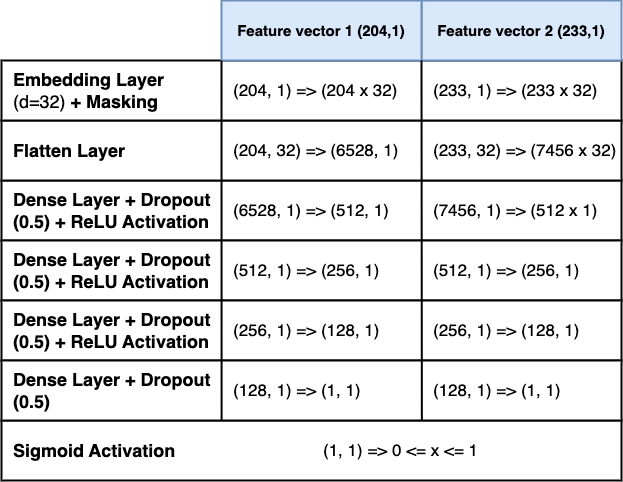
\includegraphics[width=0.7\textwidth]{images/DL.png}
  \end{center}
  \caption{This figure shows the deep learning model for both feature vectors. The different layers are shown on left column of the table. The input
  and output dimensions for each layer are shown in the other two columns.}
  \label{fig:modelStructure}
\end{figure}

By incorporating these additional features into our ML models, we aim to enhance the accuracy and effectiveness of
the tracking detection process, considering a broader range of contextual information associated with each request. 
Furthermore, every feature is known before a request is sent to the server and can be used to identify a tracking request
in real-time.

The deep neural network structure is almost identical to Castell-Uroz et al. \cite{castell2020url} and is illustrated in Fig-\ref{fig:modelStructure}.
The differences come from the different activation
function and the different input and output vector dimensions due to the different feature vectors. As Castell-Uroz et al. we use an embedding layer to reduce the bias between the numerical values of the embedded URL string. This embedded 
representation then gets flattened into a one dimensional vector and put into the four dense layers. Each dense layer has a dropout rate of 50\% to reduce
overfitting and a ReLU\footnote{Relu} activation function. The last dense layer gets activated by a Sigmoid\footnote{Sigmoid} function to generate an output
between zero and one.

By using the neural network structure of Castell-Uroz et al. we hope to achieve similar or better accuracy results with 
the newly crafted feature vector designs. However, it could be possible that the network architecture is not optimal
for the desired output and does not fit the different feature vectors. There is a chance that a better architecture could 
lead to a better accuracy result and therefore would better fit the real-time application of the model.

\subsection{Training-Data}

Selecting the appropriate training-data is a crucial step in the training of neural networks. The quality and representativeness 
of the training data directly impact the performance and generalization ability of the network.

The utilization of the model in a real-time web environment necessitates the careful selection of the training dataset.
In our study, we sought to procure a dataset that aligns with the dynamics and characteristics of real-time web browsing.
To achieve this, we turned to a comprehensive web crawl conducted by Raschke \cite{raschke_philip_2022_7123945}, which involved the exploration and collection
of data from the Tranco top 10K websites using the Chrome browser.

The choice of using a Chrome crawl dataset by Raschke holds several advantages for our model's training. Firstly, it is performed 
using the \emph{t.ex extension} \cite{9972261}, which is a cross browser extension and therefore runs in the same environment as our
application. Secondly, Chrome is one of the most widely used web browsers globally, making it a representative platform for
capturing the diverse range of web activities and behaviors.

Furthermore, the Chrome browser by default does not have any tracking protection associated. This leads to more tracking requests being executed
during the crawl which gives great potential for training a neural network. The dataset comes with 901,012 HTTP requests and responses all in JSON
format and a label to identify tracking requests from non tracking requests. Moreover, the dataset has been successfully used by Raschke et al. \cite{raschke2023}
to train a different tracker detection classifier.

For these reason we decided to use this dataset \cite{raschke_philip_2022_7123945} to train our models and further on use these models
in the real-time application.

\subsection{Real-time Application}

For our real-time application, we focused on creating a cross browser extension. This comes close to current solutions in this area 
and provides a familiar entry point for users. 

\begin{figure}[ht!]
  \begin{center}
    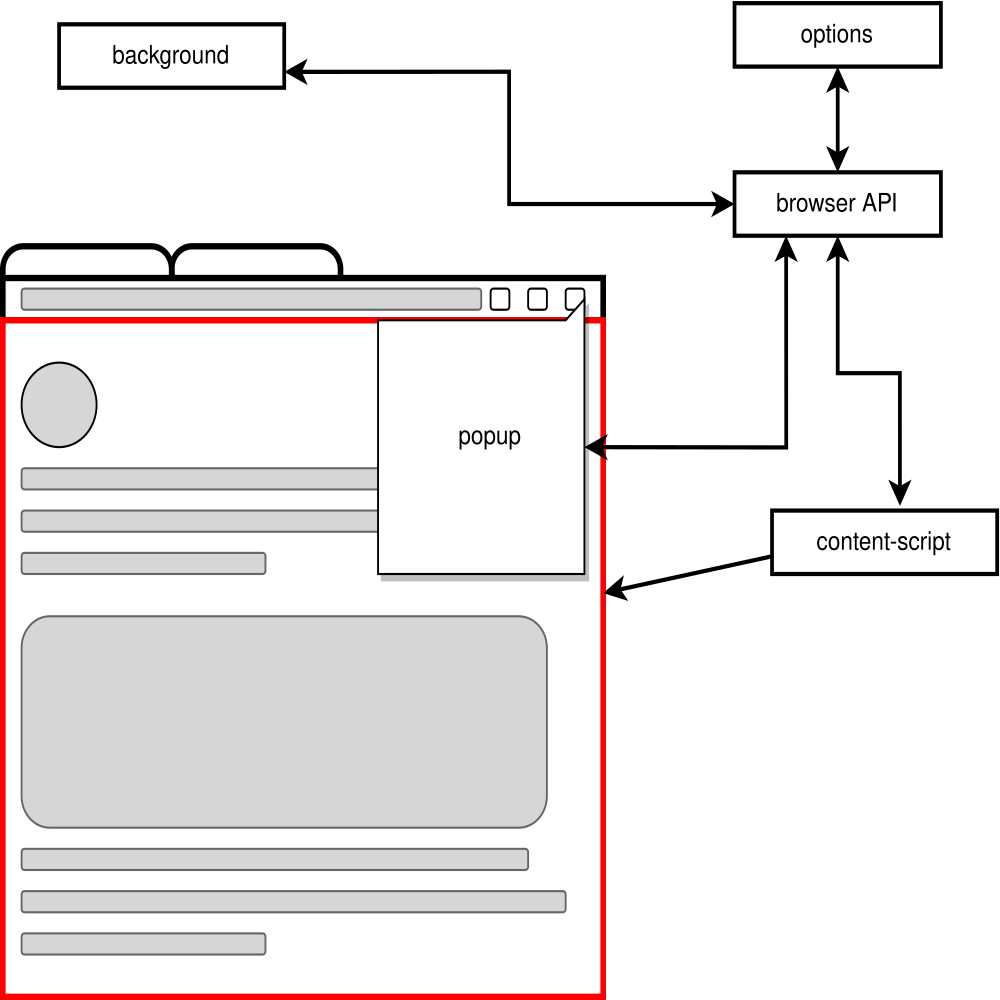
\includegraphics[width=0.75\textwidth]{images/ExtensionOverview.png}
  \end{center}
  \caption{This figure shows the structure of a web extension and its most important components. There are user interface components which 
  can be used to communicate with the user of the extension such as the popup or the options page. Additionally, there is the content-script
which can be injected into each HTML page visited by the browser and the background page which can be used to implement the business logic of the extension. All the parts of the 
extension can communicate over the API provided by the browser.}
  \label{fig:extOver}
\end{figure}

Browser extensions are event based programs which can be used to enhance the browsing
experience. Moreover, browsers provide an API which can be used by the extension programmer to interact with the browser with JavaScript.
This API can then be used to for example block HTTP requests before they get sent to the server.

As shown in Fig-\ref{fig:extOver} a web extension may consist of a \emph{background} page, a \emph{popup}, \emph{option} pages and
content-scripts. Once the background script is loaded it can attach to various browser events and react accordingly. The browser API
provides numerous events \cite{browserApi} including events that allow to read and intercept HTTP requests. Another tool is  
\emph{content-scripts} which get directly injected every web page opened in the browser and can modify its content using
JavaScript. A web extension has two methods communicating with the user through a dedicated user interface. Firstly, it is possible
to provide a popup page to display information or controls. Secondly, it is possible to host an option-page or static HTML serving. This can
be used to give the user more detailed options or when more screen space is needed.

We want to utilize the advantages of using a web extension as a real-time tracking blocker. Therefore, we implement a background script
which attaches to the \emph{onBeforeRequest} event to gather information about the request such as the \emph{requestId} and the source URL 
which initiated the request. Moreover, we also attach to the \emph{onBeforeSendHeaders} event which can be used to block a request and holds
information about the request headers. With this information we then construct a feature vector and pass it to our ML model and cancel the 
request depending on the models' confidence. 

Furthermore, to improve usability we implement a popup to show the user the amount of trackers detected on a certain website and show
each request with the according confidence. Moreover, the user is able to regulate the threshold on which a request is determined a 
tracking request, and it is possible to enable or disable the blocking of web requests. The default confidence on which a request
is deemed a tracking is set to 80\%.

The implementation of this application heavily relies on \emph{tensorflow.js} \cite{tensorflowJs} which is a library to port ML models to
JavaScript. This way we can calculate the feature vector and pass it to the TensorFlow layers model. This is extremely
performant as tensorflowjs uses WebAssembly to calculate the model and is an important factor in the real-time ability of this application.
With this concept, we meet the real-time criterion and hope to provide a seamless user-experience.

\subsection{Infrastructure}

As the web industry grows with rapid pace, also web tracker change in structure and technique. This could lead to the model being 
outdated as the training data is from a specific time. Another infrastructural problem is the use of TPLs as the ground truth. As mentioned
before these lists are error prune on often just hide certain elements from the DOM. For that reason it is important to gather better 
training data with better labels. For that reason we also implemented an infrastructure to keep the model up to date and to enable user to
provide training data with custom labels.
\begin{figure}
  \begin{center}
    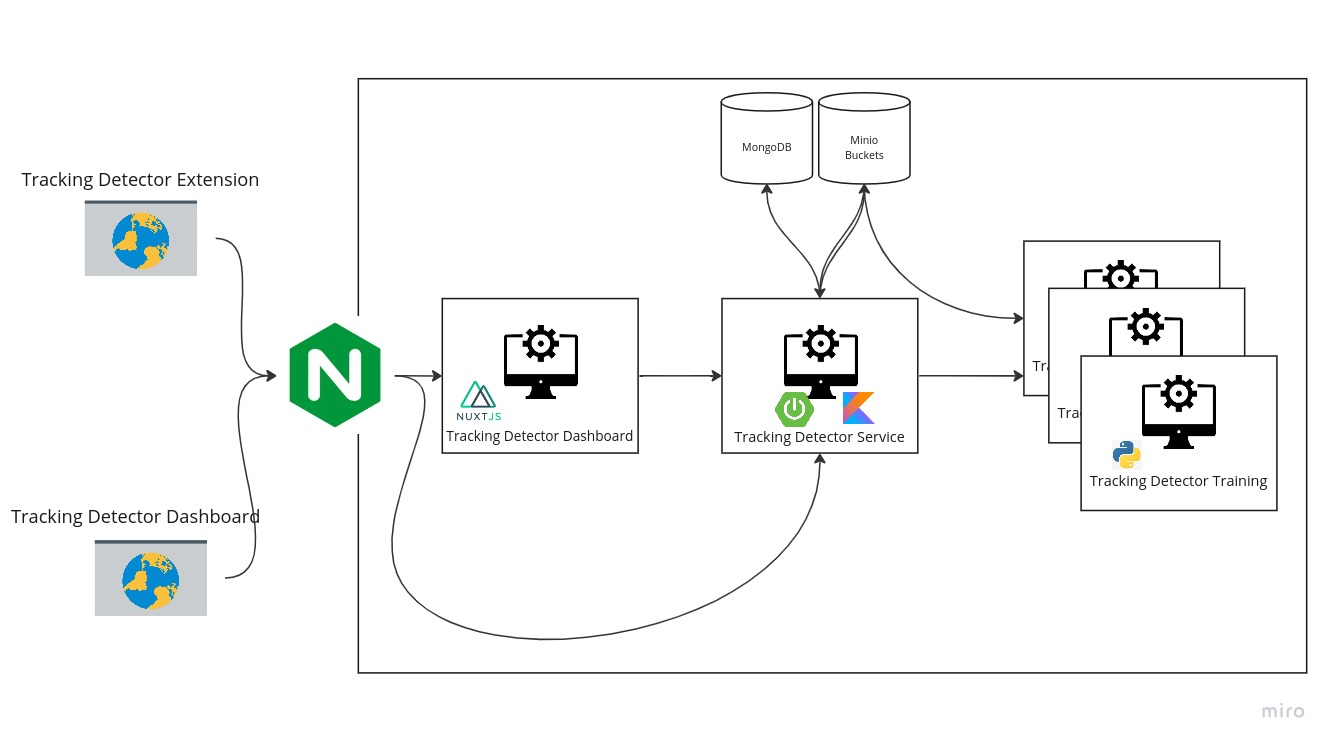
\includegraphics[width=1\textwidth]{images/TrackingDetectorInfra.jpg}
  \end{center}
  \caption{This figure shows the architecture of the whole application. As for the client side we have the web extension and an admin panel to 
  monitor the learning rate. Every endpoint proxies through a NGINX gateway. The main service is in charge of storing new data into the training dataset and 
  to host the trained models. Furthermore, it is includes a job architecture which allows running different jobs based on a CRON pattern. For data storage there is 
  a bucket storage from \emph{MinIO} and a \emph{MongoDB} to hold the data the main service servers and modifies. Finally, there are multiple training services which are Python based
  these get triggered by the main service using \emph{XMLRPC}.
  }
  \label{fig:tdInfra}
\end{figure}

As shown in Fig-\ref{fig:tdInfra} a lot of thought went into the creation of a suitable backend for the web extension. The goal of that
backend is to provide a simple way to train and deploy new ML models to the user of the web extension. The complete backend is divided into
three main services. The \emph{Tracking-Detector-Dashboard} is the admin panel which allows the admin to monitor learning rates and export 
training datasets. Through this panel it is also possible to trigger the job based architecture in the \emph{Tracking-Detector-Service}.

Another important aspect of this architecture is the storage of data within this system. For that there are two storage components within this
architecture. Firstly, the MongoDB is in charge of storing the raw browsing data of the clients and to store the ML model definitions which get 
trained. Furthermore, the statistics of each training run get stored in that database. The second storage component is a MinIO bucket storage service.
This storage is utilized to export the raw training-data into easy to process CSV files which can be used to train the models. Moreover, the trained model
binaries get stored in that storage service.

Besides, the centerpiece of this backend is the \emph{Tracking-Detector-Service}. This service is in charge of processing new data points 
submitted by the users of the web extension and to gather them into a dataset which gets exported to the MinIO file storage. It also stores 
the original representation of the data points into a MongoDB such that any dataset representation can be created. Additionally, this service
is in charge of serving the trained models to the clients, it does that by serving the stored models directly out of the MinIO storage buckets.
This service is implemented in Kotlin and uses the Spring Boot framework to create a multithreaded server environment. This framework has been choosen
because of its testability and performance.

Furthermore, the training of the models is done on one of the multiple \emph{Tracking-Detector-Training} services. These services are
lightweight XMLRPC server implemented in Python. The training gets started by a XMLRPC call to one of the services. After that, the service
grabs the training data from the MinIO storage bucket and compiles the ML model from the information provided by the XMLRPC call. It then starts
training the model and returns the model metrics to the \emph{Tracking-Detector-Service}.

As for the usability, we decided to wrap every component into a docker container and host the whole infrastructure in a \emph{docker-compose}
file which makes it easy to set up. Furthermore, this architecture can be used for all kind of ML based applications as the jobs are simple to extend 
and the creation of new models can be done via the admin panel. With this backend solution we hope to create an application that continuously creates
better models and serves them to the clients. Furthermore, we hope to simplify the process of gathering training data and to create a better
ground truth in the web tracking field.

\subsection{Limitations}

However, there are limitations to this approach. The selected features may not be optimal for the problem and should be evaluated.
This could be done by generating variations of feature vectors using all the available features before a request is sent to the server.
After that, a grid search could be implemented to validate which feature vector fits the problem best. 

Furthermore, the same problem applies to the model. The neural network structure may not be optimal for the given use case and could also
be optimized with a grid search. This might lead to performance gains. Another more generic dataset could be used to create a better generalized
model which could lead to a better performance in the real-time application causing less site breakages.

\section{Methodology}

In this section, we outline the methodology we will employ to evaluate our models and real-time application for web tracker detection.
The methodology encompasses data collection, model training, evaluation metrics, and real-time application evaluation. By following
rigorous scientific methods, we aim to ensure the reliability, accuracy, and practicality of our models and application.

\subsection{Data Collection}
To gather the necessary data for evaluating our models and real-time application, we will utilize a combination of approaches.
This will involve conducting web crawls using browsers such as Chrome and Brave. Through these web crawls,
we will collect a diverse set of web pages representing various domains. These crawls will be performed with Chrome without extensions,
Chrome with the first model, Chrome with the second model, Chrome with both models and a Brave which has build in ad and tracker blocking.
The crawler will crawl the Tranco Top 1K websites and generate a browsing graph which includes the visited domains and the HTTP request
performed on each node.

\subsection{Model Training}
The training process will involve preprocessing the dataset, including features extraction and
transformation into a suitable format for training the neural network models. We will use the model architecture by Castell-Uroz et al. \cite{castell2020url}.
To ensure the generalizability of our models, we will employ cross-validation techniques, such as k-fold cross-validation,
to assess their performance on different subsets of the data.

\subsection{Evaluation Metrics}
To evaluate the performance of our models, we will employ standard evaluation metrics commonly used in machine learning
classification tasks. These metrics include accuracy, precision, recall, F1-score, false positive rate, and false negative rate.
Accuracy will measure the overall correctness of our models in identifying web trackers. Precision, recall, and F1-score will provide
insights into the model's ability to accurately classify web trackers and non-trackers. The false positive rate and false negative
rate will help assess the model's performance in minimizing false positives and false negatives, which directly impact user
experience and privacy.

\subsection{Real-time Application Evaluation}
In order to evaluate the performance of our real-time web tracker detection application, we will evaluate the gathered data 
and look at the browsing graphs to determine the difference in the browsing experience.
Additionally, we will measure the impact of the web extension on browsing performance, such as page load times and
resource consumption, to ensure minimal disruption to the user's browsing experience.





